\documentclass[10pt,a4paper,hidelinks]{article}
\usepackage{polyglossia}
\setdefaultlanguage{english}
\usepackage{amsmath}
\usepackage{cite}
\usepackage{amsfonts}
\usepackage{amssymb}
\usepackage{makeidx}

\usepackage{hyperref}
\newcommand{\algorithmautorefname}{algorithm}

\usepackage{cite}

\usepackage{listings}
\lstset{
	tabsize=4,
	morekeywords={forelem}
}

\usepackage{algorithmicx}
\usepackage{algpseudocode}
\usepackage{algorithm}

\usepackage{datetime}

\usepackage{tikz}
\usetikzlibrary{shapes,arrows}

% Preamble for the LIACS style
\setlength{\textheight}{24.7cm}
\setlength{\textwidth}{16cm}
\setlength{\unitlength}{1mm}
\setlength{\topskip}{1truecm}
\topmargin 280mm \advance \topmargin -\textheight
\divide \topmargin by 2 \advance \topmargin -1in
\headheight 0pt \headsep 0pt
\leftmargin 210mm \advance \leftmargin -\textwidth
\divide \leftmargin by 2 \advance \leftmargin -1in
\oddsidemargin \leftmargin \evensidemargin \leftmargin
\parindent=0pt
\frenchspacing

\newcommand{\bree}[1]{\makebox[4.1cm][l]{#1:}}

\begin{document}


%No page number
\thispagestyle{empty}
\sf 

\begin{tabular}[t]{p{1.5cm}@{\hspace{4mm}\vrule width 1.5pt\hspace{4mm}}l}
%Logo Leiden University
\makebox(0,0)[t]{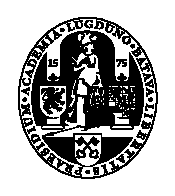
\includegraphics{ullogo.eps}}
&
\begin{minipage}[t]{14cm}
\begin{Huge}
\vspace*{0.4cm}
\textbf{Universiteit Leiden}
\\[2ex]
\textbf{Opleiding Informatica}
\end{Huge}

\vspace*{4cm}

\begin{Large}
% --> Here your title
\hfill Utilizing a tuple based optimization framework
\vspace*{3mm}

\hfill for graph algorithms

\vspace*{5.5cm}


%% --> Add your data here!
\bree{Name}%
Bert Peters
%\\
%\bree{Studentnr}%
%nnnnnnnn
\\[1ex]
\bree{Date}%
\today
\\[1ex]
\bree{1st supervisor}%
Harry Wijshoff
\\ 
\bree{2nd supervisor}%
Kris Rietveld
\end{Large}


\begin{large}
\vspace*{3.5cm}
BACHELOR THESIS

\vspace*{5mm}
Leiden Institute of Advanced Computer Science (LIACS)\\
Leiden University\\
Niels Bohrweg 1\\
2333 CA Leiden\\
The Netherlands
\end{large}

\end{minipage}
\end{tabular}

\tableofcontents

\section{Introduction}

\subsection{The problem}

The problem we intend to solve is the max flow min cut problem. It was first formulated in 1954 as a way of modelling Soviet railway flow\cite{HarrisRoss}. The problem asks what, given a graph $(V,E)$ in which every edge has a flow capacity $c$, is the maximum flow from a given source to a given sink. For example, the in the graph shown in figure~\ref{fig:simple-graph} has a maximum flow of 14, utilizing the capacities as shown.

\begin{figure}[h]
\centering
\begin{tikzpicture}[->,>=stealth',shorten >=1pt,auto,node distance=3cm,
  thick,main node/.style={circle,fill=blue!20,draw,font=\sffamily\Large\bfseries}]

  \node[main node] (1) {s};
  \node[main node] (2) [above right of=1] {a};
  \node[main node] (3) [right of=2] {b};
  \node[main node] (4) [below right of=1] {c};
  \node[main node] (5) [right of=4] {d};
  \node[main node] (6) [above right of=5] {t};

  \path[every node/.style={font=\sffamily\small}]
    (1) edge node {10/16} (2)
        edge node {4/4} (4)
    (2) edge node {10/12} (3)
    (3) edge [bend right] node [left] {3/3} (4)
        edge node {7/7} (6)
    (4) edge node {7/10} (5)
    (5) edge node {7/10} (6)
        edge [bend right] node [right] {0/5} (2)
    ;
\end{tikzpicture}
\caption{A simple graph with flows.}
\label{fig:simple-graph}
\end{figure}

It should be noted that the flow configuration for the maximum flow is not necessarily unique, although in this example it is. The only requirement is that for each node (excluding the source and the sink) the incoming flow is equal to the outgoing flow.

\subsubsection{Ford-Fulkerson algorithm}

The Ford-Fulkerson algorithm computes for a given directed graph of edges $(u, v, c)$ with $u$ and $v$ nodes and $c$ the capacity for the edge, the maximum ``flow'' from a given source $s$ to a sink $t$, given that the flow of an edge $e$ can never exceed its capacity. The algorithm assumes that

\begin{itemize}
\item there are no parallel edges, meaning that 
$$
\forall e_1 (u_1, v_1, c_1), e_2(u_2, v_2, c_2): e_1 \neq e_2 \implies u_1 \neq u_2 \land v_1 \neq v_2
$$, and
\item there are no self loops, meaning that
$$
\nexists e (u, v, c): u = v
$$
\end{itemize}

The former condition is easily satisfied, as we can just merge two parallel edges by adding their respective capacities. The latter we can satisfy by can completely ignoring any self loops. This is valid, as self loops do not contribute to the total flow.

The algorithm works as follows. We define $f(u,v)$ and $c(u, v)$ as the flow and capacity respectively from $u$ to $v$. For all $u$ and $v$, we initialize $f(u, v)$ as zero. For all edges $(u, v, c)$, we define $c(u, v) = c$ and for all other combinations, we define $c(u, v) = 0$.

\begin{algorithm}
\caption{A pseudo-code representation of the Ford-Fulkerson algorithm}
\label{algo:ford-fulkerson}
\begin{algorithmic}

\Function{FindPath}{$source, destination, path$}
	\If{$source = destination$}
		\State \Return{$path$}
	\Else
		\ForAll{$e : e \in E \land e.u = source \land e \notin path \land f(e.u, e.v) < c(e.u, e.v)$}
			\State $newPath \gets$ \Call{FindPath}{$e.v, destination, path \cup e$}
			\If{$newPath \neq \emptyset$}
				\State \Return{$newPath$}
			\EndIf
		\EndFor
		\State \Return{$\emptyset$}
	\EndIf
\EndFunction
\State
\While{there is a useful path from $s$ to $t$}
	\State $path \gets$ \Call{FindPath}{$s, t, \emptyset$}
	\State $\delta \gets \min(c(e.u, e.v) - f(e.u, e.v) \forall e \in path$
	\ForAll{$e \in path$}
		\State $f(e.u, e.v) \gets f(e.u, e.v) + \delta$
		\State $f(e.v, e.u) \gets f(e.v, e.u) - \delta$
	\EndFor
\EndWhile
\State $maxflow \gets \sum\limits_{e : e.v = t} f(e.u, e.v)$
	
\end{algorithmic}
\end{algorithm}

\subsubsection{Push-Relabel algorithm}

We define the set of nodes, $V$, and the set of edges $E$. Furthermore, we define the function $\Delta(u)$ which denotes the current excess flow at node $u$, and $F(u, v)$ and $C(u, v)$, which denote the current flow and the flow capacity from $u$ to $v$ respectively. Both start at $0$ if the edge does not exist.

A new property that is used, is the height function $H(u)$, which holds the current height for a given node. This height function is used to enforce an ordering.

The algorithm has two operations. The \textsc{Push} operation pushes excess flow from a node $u$ to a connected node $v$. It is allowed only when $H(u) = H(v) + 1$. If no valid push is possible, a node must be relabeled with the \textsc{Relabel} operation. This method increases $H(u)$ to the minimum level so that a new push is allowed.

The algorithm starts by performing a satisfying push on the source node, which fully uses all outgoing edges on that node. After that, the algorithm attempts to either push the excess flow to the sink, or, if it is not possible to push, relabels the node. When there are no longer any nodes with an excess flow, the algorithm is finished and the maximum flow can be calculated by summing the flow coming into the sink $t$ or the flow going out of the source $s$. A pseudo-code implementation can be seen in algorithm~\autoref{algo:push-relabel}.

\begin{algorithm}
\caption{A pseudo-code implementation of the generic Push-Relabel algorithm}
\label{algo:push-relabel}

\begin{algorithmic}
\Function{Push}{$e, amount$}
	\State $\delta \gets \min(amount, C(e.u, e.v) - F(e.u, e.v))$
	\State $\Delta(e.u) \gets \Delta(e.u) - \delta$
	\State $\Delta(e.v) \gets \Delta(e.v) + \delta$
	\State $F(e.u, e.v) \gets F(e.u, e.v) + \delta$
	\State $F(e.v, e.u) \gets F(e.v, e.u) - \delta$
\EndFunction

\State

\Function{Relabel}{$u$}
	\State $H(u) \gets \min(H(v) : F(u, v) < C(u, v)) + 1$
\EndFunction

\State

\ForAll{$e : e \in E \land e.u = s$}
	\State \Call{Push}{$e, \infty$}
\EndFor

\State

\State $H(s) \gets |V|$
\State $H(V \setminus s) \gets 0$

\State

\While{$\exists u : u \in V \setminus t \land \Delta(u) > 0$}
	\If{$\exists e : e \in E \land e.u = u \land C(e.u, e.v) > F(e.u, e.v) \land H(e.u) = H(e.v) + 1$}
		\State \Call{Push}{$e, \Delta(u)$}
	\Else
		\State \Call{Relabel}{$u$}
	\EndIf
\EndWhile

\State

\State $maxflow \gets \sum\limits_{e : e.v = t} F(e.u, e.v)$
\end{algorithmic}
\end{algorithm}

\subsection{The forelem language}

For this research, we will use the forelem framework \cite{Rietveld} to represent a general algorithm for the max flow problem. In this framework the data is expressed as several unordered sets of tuples and the algorithm can be expressed as an unordered loop with some operations over those tuples. To denote.

As an example, we take a set of tuples \texttt{A} with two values, \texttt{part1} and \texttt{part2}, and we want to calculate the sum of $\text{\texttt{part1}} \times \text{\texttt{part2}}$, then an algorithm could be expressed as in algorithm \ref{algo:forelem-sum}. In this algorithm, \texttt{pA} notates the set of indices for the tuple set A, with no guarantees of ordering of any kind. All that is known is that a tuple can be queried with an index. This leaves a compiler free to choose a data structure which does not have a strict ordering, like a set, or a structure without random access, like a linked list.

Once an algorithm is formatted that way, it can be materialized, transformed and concretisised into a regular programming language (such as C or Python) to be compiled and executed normally. The actual transformations can be found in chapter 9 sections 4 to 7 of \cite{Rietveld} but is out of the scope of this thesis.

\begin{algorithm}
\caption{\emph{forelem} algorithm for summing the products of a set of tuples}
\label{algo:forelem-sum}
\begin{lstlisting}[mathescape]
sum = 0
forelem (i; i $\in$ pA)
	sum = sum + A[i].part1 $\times$ A[i].part2
\end{lstlisting}
\end{algorithm}

\bibliography{bibliography}
\bibliographystyle{plain}

\end{document}
